El problema de síntesis de controlador ya tiene una solución clásica, por lo que la dificultad del trabajo no consistió en desarrollar un algoritmo que detectara estados ganadores y perdedores de un LTS totalmente explorado. 

El conflicto reside en que al componer distintos DES, la cantidad de estados de la composición es exponencial respecto de los estados en los componentes. Esto es de suma relevancia ya que la solución clásica, que compone toda la planta para luego explorarla, tiene un límite de escalabilidad en el cual la composición de la planta llega al límite de tiempo o memoria, y nunca se llega a la exploración.

Para combatir esto, la exploración on-the-fly, presentada en \textcolor{red}{REF DANY}, clasifica estados como ganadores o perdedores durante la composición. Se espera que con esto sea posible, en primer lugar, cortar la exploración de una rama de la planta que ya se sabe que es perdedora o ganadora, reduciendo así la memoria y tiempo necesarios. Pero más aún, si el estado inicial fuera marcado como ganador o perdedor antes de la composición completa de la planta, ni siquiera sería necesario completar el proceso de composición.

\begin{lstlisting}[language={pseudocode},label={lst:basic_on-the-fly},caption={Algoritmo on-the-fly básico},float=ht]
Algorithm basicOTF-Exploration($E, A_E^C$):
    $\initial$ = $\<\init{e}^0,\ldots,\init{e}^n\>$
    $\structure \subseteq E$
    until seguroGanaOPierde($\initial$):
        expandirES()
        computarGanadoresYPerdedores($\structure$)
    return armarControlador($\initial$)
        
\end{lstlisting}

En el listing \ref{lst:basic_on-the-fly} mostramos la estructura básica de este método. Trabajando sobre la parte de la planta compuesta hasta el momento (estructura explorada, Explored Structure, $\structure$), se expande $\structure$ consiguiendo nueva información hasta que sea seguro si el estado inicial es ganador o perdedor en $E$. Al llegar a esta conclusión se retorna el controlador para $\initial$ en $E$ o se notifica que no es controlable.

Puede haber muchas variantes de cada una de estas partes, cómo se expande, cómo se computan nuevos ganadores y perdedores, etc. En particular, nuestro enfoque se muestra en el listing \ref{lst:on-the-fly} y consiste en ir agregando una transición a la vez a la parte conocida de la planta, y en cada paso ver si esta nueva transición permite concluir que un estado es ganador o perdedor. Si algún nuevo estado se clasifica como ganador  o perdedor, se propaga esta información a sus antecesores, posiblemente marcándolos a su vez como ganadores o perdedores, respectivamente.

A medida que exploramos mantenemos dos conjuntos de estados de $\structure$ ($\Goals$ y $\Errors$) para los cuáles ya se tiene una conclusión, es decir, se sabe que son ganadores (o perdedores) en $E$.

Como se demostrará en el capítulo \ref{chpt:dcs}, al expandir $\structure$ con una transición a la vez $(e,\l,e')$, a menos que $e'$ ya fuera un ganador/perdedor entonces sólo puede haber nueva información si existe un loop entre $e$ y $e'$. Ésto permite optimizar la detección de nuevos ganadores/perdedores en lugar de ejecutar un algoritmo clásico sobre todo $\structure$.

En el peor caso, no se pudo concluir nada antes de componer la planta en su totalidad, se perdió tiempo en los puntos fijos, intentando clasificar estados, y se realiza una última vez el algoritmo clásico con la planta totalmente explorada. Esto garantiza la completitud del algoritmo, como se detalla en mayor profundidad en el capítulo~\ref{chpt:dcs}.

\begin{lstlisting}[language={pseudocode},label={lst:on-the-fly},caption={Nuestro enfoque on-the-fly},float=ht]
Algorithm genericOTF-Exploration($E, A_E^C$):
   $\initial$ = $\<\init{e}^0,\ldots,\init{e}^n\>$
   $\Goals = \Errors = \emptyset$
   $\structure = initial$ //la parte conocida de la planta
   while $initial \notin \Goals \cup \Errors$:
     $(e,\l,e') = $proxTransicion($\structure, heuristica$)
     expandirES($\structure,(e,\l,e')$)
     if $e' \in \Errors$:
       propagarError($e'$)
     else if $e' \in \Goals$:
       propagarGoal($e'$)
     else if isLoop($e,e'$):
       if nuevoLoopGanador($e,e'$):
         propagarGoal($e'$)
       else if nuevoLoopPerdedor($e,e'$):
         propagarError($e'$)
         
   if $initial \in \Goals$:
     return armarControlador($\Goals$)
   else:
     return "UNREALIZABLE"  
\end{lstlisting}

Para incrementar las ramas podadas se utiliza una heurística de exploración Best First Search \cite{tesisDani} que busca ganar controlablemente o perder no controlablemente, para garantizar con la menor exploración posible que el estado actual es ganador o perdedor.

Una heurística no presenta garantía de resultados perfectos, más bien da una recomendación. Son ampliamante utilizadas al optimizar, pero es importante que la correctitud de los algoritmos no dependan de estas recomendaciones, ya que por su misma naturaleza no tienen garantías fuertes.

A continuación presentamos los puntos más delicados de la exploración on-the-fly, y presentamos las ideas que moldearon nuestro algoritmo para resolver estos puntos conflictivos.

En todos los gráficos siguientes vamos a utilizar las letras $c$, $u$, para denotar si una transición es controlable o no, respectivamente; en caso de no especificar letra para una transición es porque su controlabilidad no afecta el resultado del ejemplo.

\section{Marcado explícito de errores}\label{marcarErrores}

% FALENCIAS AL ENCONTRAR ERRORES
Un estado deadlock (sin transiciones de salida) es obviamente un error, ya que si caemos en él no podemos alcanzar nunca un estado marcado. Ahora, ¿qué pasa si tenemos un conjunto de estados conectados entre sí pero sin conexión a otros fuera del conjunto?. Depende si existe un estado marcado dentro del conjunto o no, de no haberlo no tenemos forma de alcanzar uno (ya que no podemos salir del conjunto). 

Es el caso de la figura \ref{fig:falenciasErrores}, el conjunto o rama $B$ fue totalmente explorado y no contiene ningún estado marcado. En éste momento es importante que agreguemos todos los estados de $B$ a $\Errors$, de no hacerlo podríamos incurrir en un error al propagar goal desde otra rama. Es decir, si se mira primero la rama de abajo y no lo marcamos como error (a pesar de estar completamente explorado), entonces al mirar la de arriba diremos que es goal y propagaremos dicha información, equivocadamente, más allá de $e$. 

Éste problema se evita respetando el invariante presentado en la propiedad \ref{def:invariant}, como se explica en \ref{sct:enfoque}.

\begin{figure}[htb]
	\centering
	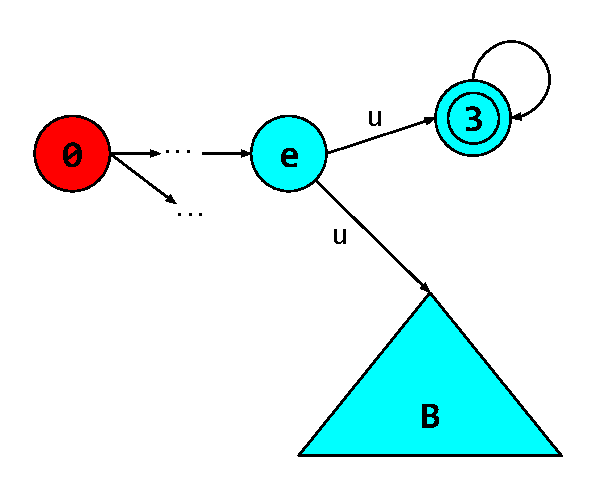
\includegraphics[width=\linewidth/2]{figures/FalenciasErrores.pdf}
	\caption{Caso sub-autómata completamente explorado (B), sin marcados dentro.}
	\label{fig:falenciasErrores}
\end{figure}

\section{Propagación local vs por conjuntos}\label{propagacionLocal}

% PROPAGACION LOCAL
Una vez obtenido un resultado necesitamos propagarlo hacia los estados ancestros; necesitamos saber, para cada estado, si es posible sacar una conclusión dada la nueva información. Muchas veces es imposible hacerlo teniendo una mirada local, analizando solo un estado a la vez, ya que se pierde información sobre lo que sucede dentro del ``conjunto'' de ancestros vecinos.

Por ejemplo en el caso de la figura \ref{fig:propagarError}, hay un loop controlable entre dos estados, el cual se explora primero, y uno de ellos va controlablemente a un error. Debe habilitarse alguna controlable saliente del estado 2 (caso contrario sería un deadlock), pero ninguna lleva a un estado ganador, por ende la planta es no controlable. Pero según la mirada local nunca se concluiría que los estados [1, 2] son errores, porque ambos tienen \textit{una forma de escapar del error}, el otro estado del loop, y no se sabe que ese otro estado está en la misma situación. 

Equivalentemente la mirada local tampoco funciona propagando $\Goals$, en la figura \ref{fig:propagarGoal} se puede ver un ejemplo. El estado $2$ llega al estado marcado $3$ pero no puede forzarlo, sin importar si la transición a $3$ es controlable o no ya que tiene una transición no controlable a $1$. Como $1$ sólo puede volver a $2$ ésta situación no nos molestaría (por ser non-blocking) y el modelo debería ser controlable. Pero si miramos localmente al propagar $Goal$ desde $3$, \textit{no sabemos dónde nos lleva la transición no controlable de 2 a 1}, y deberíamos suponer lo peor, sin poder marcar a 2 como ganador.

Entonces una mirada local no funciona a la hora de propagar. Pero ¿qué conjunto de ancestros vecinos deberíamos tomar? es difícil decidir dónde hacer el corte; son muchos casos y no se puede, localmente, distinguirlos a todos. Por ende es necesario una propagación más inteligente, con una mirada global del conjunto de ancestros.

Como se detallará en el próximo capítulo, al momento de propagar resultados, tanto estados $\Goals$ como $\Errors$ recurrimos a un punto fijo. De esta forma tenemos en cuenta toda la información acumulada de los estados en cuestión. Si bien esto implica un mayor costo de cómputo, asegura la correcta propagación de información, lo que más adelante facilita, por ejemplo, la detección de ciclos perdedores.\\

\begin{figure}[htb]
	\centering
	\makebox[\linewidth][c]{%
		\begin{subfigure}[t]{.5\textwidth}
			\centering
			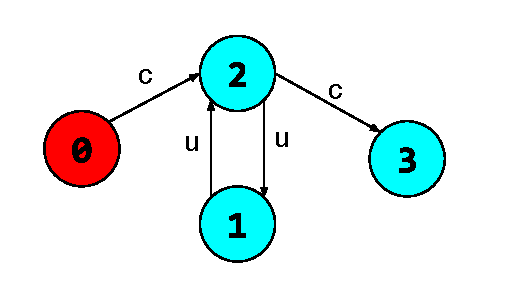
\includegraphics[width=\linewidth]{figures/PropagarError.pdf}  
			\caption{Propagar errores}
			\label{fig:propagarError}
		\end{subfigure}
		\begin{subfigure}[t]{.5\textwidth}
			\centering
			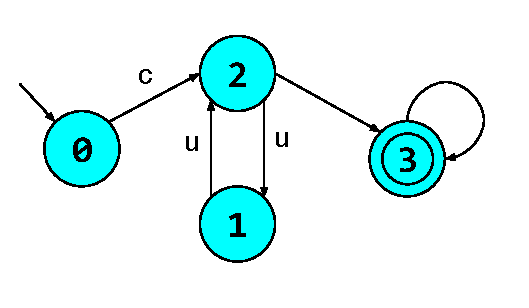
\includegraphics[width=\linewidth]{figures/PropagarGoal.pdf}  
			\caption{Propagar goals}
			\label{fig:propagarGoal}
		\end{subfigure}
	}
	\caption{Problemas de propagación local.}
	\label{fig:propagacionLocal}
\end{figure}

% \subsection{Completitud de exploración}

% FALTA DE COMPLETITUD
% Con lo explicado hasta el momento queda claro que, teniendo una conclusión para cada uno de los estados hijos del inicial, podemos definir si el problema es o no controlable. Esto depende fuertemente que dichas conclusiones sean correctas y no haya problemas de propagación. De no ser así nos puede ocurrir que se termine la exploración prematuramente y se devuelvan resultados equivocados.

% 
% Un ejemplo particular puede verse en la figura \ref{fig:faltaCompletitud}. Si tuviésemos los errores explicados en las sub-secciones anteriores se terminaría la exploración al ver el estado
% 
% al terminar la exploración se concluyó que era controlable, sin embargo al querer construir el controlador se descubre que el estado $1$ tiene una no controlable por explorar, devolviendo entonces que no existe controlador. 
% 
% Lo que sucedía era que al tener conclusiones erróneas y problemas de propagación había ciertos casos donde, según el algoritmo de exploración el problema era controlable pero al llegar al constructor del controlador se daba cuenta que había estados a los cuales les faltaba exploración y que, de hecho, tenían transiciones no controlables a estados sin mirar. 
% Llegado ese punto devolvía que no había controlador, cuando de seguir explorando hubiese visto que lo que faltaba era algo ganador. 

%\begin{figure}[htb]
%	\centering
%	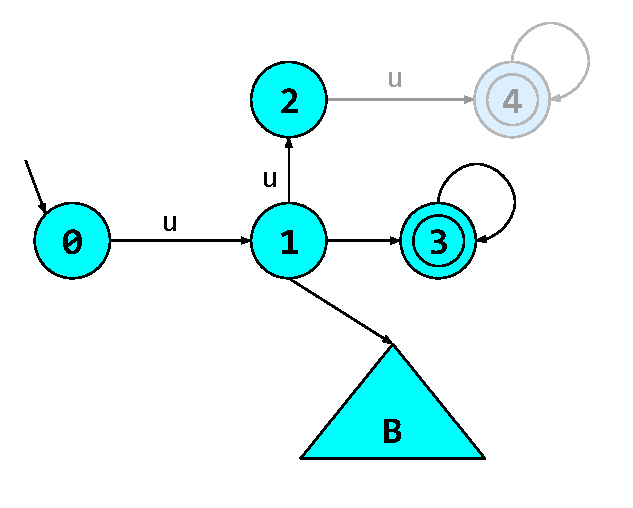
\includegraphics[width=\linewidth/2]{figures/faltaDeCompletitud.pdf}
%	\caption{Ejemplo de falta de completitud, los estados en gris son los faltantes por explorar.}
%	\label{fig:faltaCompletitud}
%\end{figure}

\section{Correcta detección de loops ganadores}

La detección de loops con estados ganadores es una pieza central para la optimización y corrección del algoritmo, y tampoco puede solucionarse con una mirada local. Es sencillo dar una descripción declarativa de los estados a encontrar (ver listing \ref{lst:viejoMCCC}) pero no resulta claro cómo implementarla. 

Luego de varios intentos más veloces pero que presentaban fallas, llegamos a la conclusión de utilizar un algoritmo de punto fijo clásico (similar a listing \ref{lst:classical}) pero con una planta reducida. Los enfoques más veloces que intentamos sí funcionaron a la hora de detectar errores y terminaron sembrando las bases para \texttt{findNewErrorsIn($loops$)}.

Como se verá más adelante, para detectar ganadores, corremos un algoritmo clásico sobre una versión pesimista de la planta explorada, que asume que toda transición no explorada es perdedora; además, de los estados ya explorados solo tomamos en cuenta un grupo reducido que forma un loop sobre la última transición explorada. Este enfoque otorga la completitud del algoritmo tradicional mientras que sostiene la eficiencia de la exploración on-the-fly.

\begin{lstlisting}[language={pseudocode},label={lst:viejoMCCC},caption={vieja descripción estados ganadores},float=ht, frame=single]
function buildMCCC($e, e'$):
let $C$ such that
$C = \{ e_i \mid (e' \runw{w}{\structure} e_i \runw{w'}{\structure} e \vee e \runw{w}{\structure} e_i \runw{w'}{\structure} e') \wedge $extendsCCC($e_i,C \cup \Goals$)$ \wedge$
$(\exists w \ldot e \runw{w}{\structure} e_m \wedge e_m \in M_E \cap (C \cup \Goals)) \}$
return $C$

function extendsCCC($e, C$):
return $(\exists \l \ldot e \step{\l}{E} e' \wedge e' \in C) \wedge (\forall \l_u \in A_U \ldot e \step{\l_u}{E} e' \Rightarrow e' \in C)$

\end{lstlisting}

\section{Agnosticismo a la heurística}

Una distinción clave del algoritmo \textit{on-the-fly} es que está dividido en dos partes. Por un lado se tiene el algoritmo de exploración responsable de que al final se llegue al resultado correcto, por el otro tenemos una heurística que le brinda la próxima transición a explorar. Ese algoritmo de exploración no puede depender de la heurística, ya que la misma no garantiza siempre elegir el mejor camino posible, sino solo la mejor aproximación que encuentre. Uno de los focos de nuestro trabajo fue en esa corrección independiente del orden de exploración de las transiciones.

El proyecto \texttt{MTSA} inicialmente contaba con dos heurísticas \texttt{Best First Search} para exploración, \textit{Monotonic Abstraction} y \textit{Ready Abstraction}. 

El inconveniente con la versión anterior del algoritmo de exploración es que había sido desarrollado en conjunto con las heurísticas. Si bien esto ayudaba a la eficiencia del mismo, generaba una dependencia del orden de observación de las transiciones, dando resultados erróneos al cambiar las recomendaciones. El nuevo enfoque no depende de la forma de explorar, por ende, da una mayor libertad de investigar a futuro nuevos criterios de evaluación para mejorar la eficiencia de la técnica sin comprometer corrección ni completitud. Esto fue útil durante el desarrollo del trabajo, ya que facilitó la inclusión de nuestras nuevas heurísticas (\texttt{Dummy} y \texttt{Breadth First Search}, ver sección \ref{chpt:heurist-nuevas}) para la experimentación.





\section{Invariante}\label{sct:invariante}

Intentando resolver el problema del marcado explícito de errores, buscamos una separación fuerte entre los estados $error \in L_E$ y los estados para los cuales no tenemos suficiente información para clasificar en este momento $\NONE$. Para esto, los lemas detallados en la sección de demostración del algoritmo aseguran que un estado marcado como ganador o perdedor lo es en la planta compuesta totalmente explorada, y nunca puede cambiar su estado.

Como se verá en la propiedad~\ref{def:invariant} del siguiente capítulo, un estado $s$ solo puede seguir sin clasificar (siendo $\NONE$) si, con los explorados hasta el momento, y siendo totalmente optimistas sobre las transiciones desconocidas no podemos asegurar que $s$ está condenado a ser perdedor (y tampoco podemos concluir que es ganador siendo pesimistas).

Al momento de haber explorado todos los descendientes de $s$, incluso si no se exploró toda la planta total, es claro que no importa si se es optimista ($\top$) o pesimista ($\bot$) para saber si $s$ es un estado ganador o perdedor, por lo que nos forzamos por nuestro invariante a clasificarlo. Con esto evitamos las ramas totalmente exploradas pero sin clasificar que traían complicaciones en la figura~\ref{fig:falenciasErrores} y solo permitimos que un estado sea $\NONE$ si tiene un camino a una transición no explorada.\\



